%----------------------------------------------------------------------------------------
%	Inställningar och dokumentkonfiguration
%----------------------------------------------------------------------------------------

\documentclass[paper=a4, fontsize=11pt]{report} % A4-sida och 11 punkters fontstorlek

\usepackage[T1]{fontenc} % 8-bitarskodning som har 256 glyfer
\usepackage[swedish]{babel} % Svenskt språk
\usepackage[utf8]{inputenc} % För svenska tecken
\usepackage{dtklogos} % Logos
\usepackage{wallpaper} % Bakgrundsbild
\usepackage{fancyhdr} % Specialsidhuvud och sidfot
\usepackage{enumerate} 
\usepackage{xifthen}% provides \isempty test
\usepackage{listings}% Code examples
\usepackage{xcolor}
\newcounter{tmpc}
\lstdefinestyle{BashInputStyle}{
  language=bash,
  basicstyle=\small\sffamily,
  numbers=left,
  numberstyle=\tiny,
  numbersep=3pt,
  frame=tb,
  columns=fullflexible,
  backgroundcolor=\color{yellow!20},
  linewidth=0.9\linewidth,
  xleftmargin=0.1\linewidth
}
% Exampels
% Inline
% \lstinline[style=BashInputStyle]´# apt-get --purge remove rubygems´.
% Multiline
% \begin{lstlisting}[style=BashInputStyle]
%    # apt-get --purge remove rubygems
% \end{lstlisting}

\pagestyle{fancyplain} % Använd sidhuvud och sidfot på alla sidor
\fancyhead[L]{Seminar 2 -- 1DV020 -- 2015 -- Server Administration} % Titel till vänster i sidhuvud
\fancyhead[C]{} % Tomt i mitten
\fancyhead[R]{} % Tomt till höger
\fancyfoot[L]{} % Tomt till vänster
\fancyfoot[C]{} % Tomt i mitten
\fancyfoot[R]{\thepage} % Sidnumrering till höger i sidfoten
\renewcommand\thesection{\arabic{section}} % Section beter sig som i dokumentklassen article

\newcommand{\win}[1]{Microsoft Windows Server\ifthenelse{\isempty{#1}}{}{ #1}}
\newcommand{\gui}[0]{``Server with a GUI''}
\newcommand{\core}[0]{Windows Server Core}
%----------------------------------------------------------------------------------------
%	TITLE SECTION
%----------------------------------------------------------------------------------------
\newcommand\BackgroundPic{
    \put(-50,-50){
    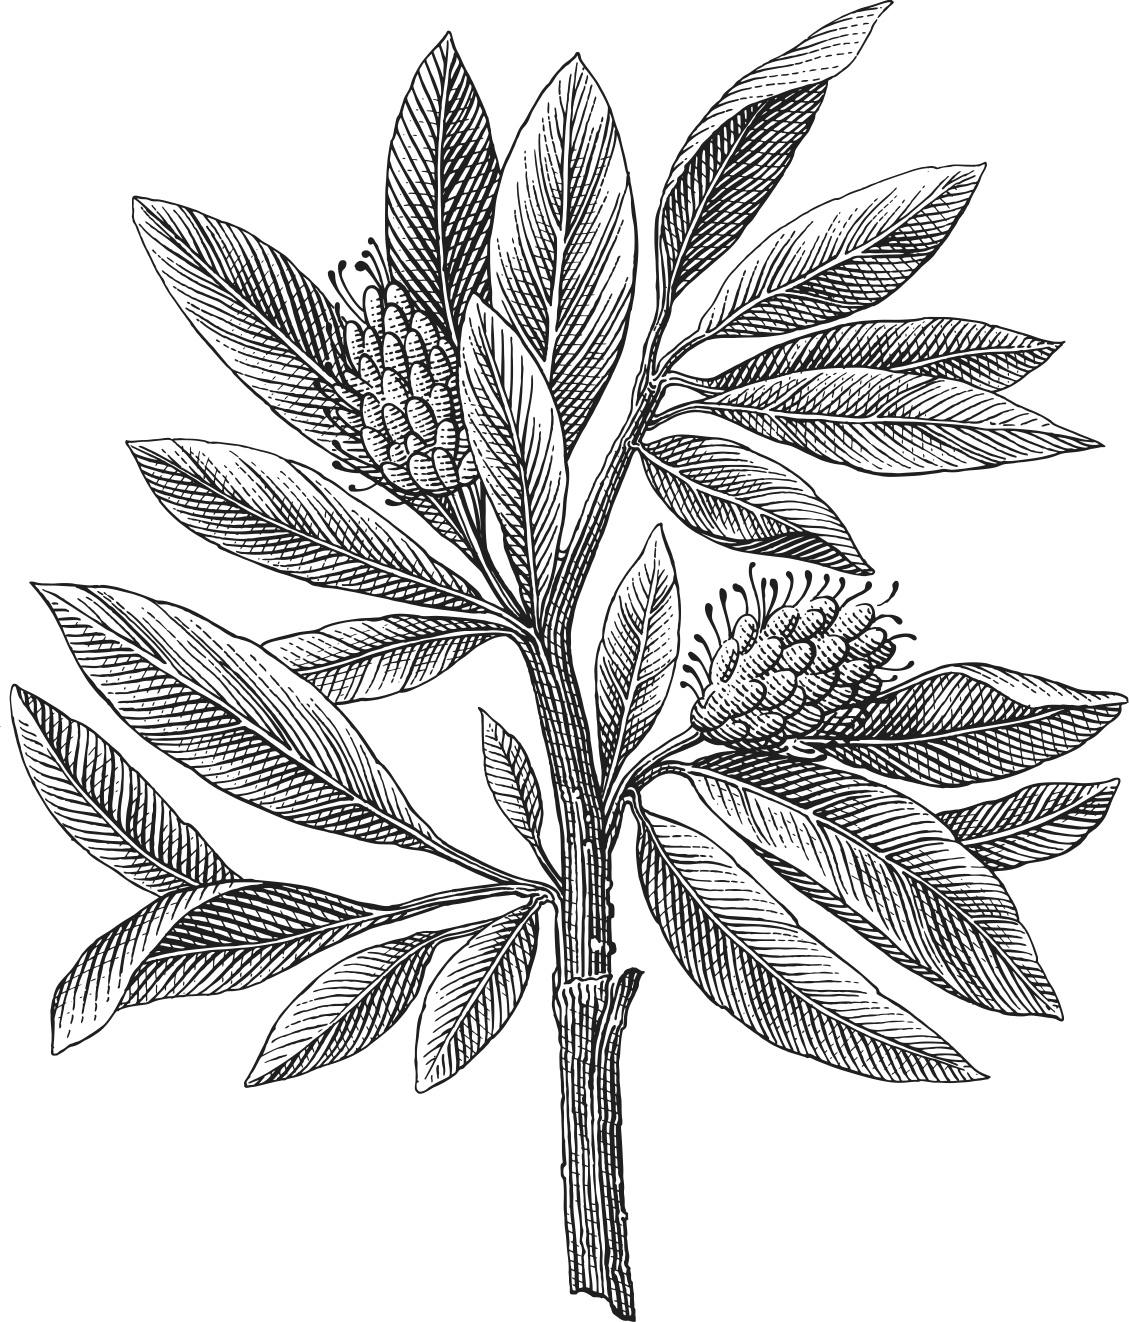
\includegraphics[keepaspectratio,scale=0.65]{lnu_etch.png} % Bakgrundsbild
    }
}
\newcommand\BackgroundPicLogo{
    \put(15,700){
    
\includegraphics[keepaspectratio,scale=0.10]{logo.png} % Logga i vänstra hörnet
    }
}

\newcommand{\horrule}[1]{\rule{\linewidth}{#1}} % Skapa hortisontell linje

\title{	\vspace{-10cm}
    \normalfont \normalsize
    \textsc{Linnaeus University} \\ [25pt] % Universitetes namn
    \horrule{0.5pt} \\[0.4cm] % Tunn linje högst upp
    \huge Seminar 2\\ % Arbetes titel
	\large \textcolor{gray}{1DV020 -- Server Administration}
    \horrule{0.5pt} \\[0.4cm] % Tunn linje längst ner
}

\author{Jacob Lindehoff} % Författarnas namn

\date{\normalsize\today} % Dagens datum

\begin{document}
  \AddToShipoutPicture*{\BackgroundPic} % Lägger in backgrundsbild på första sidan
  \AddToShipoutPicture*{\BackgroundPicLogo}
  \maketitle % Skriv ut titeln
  \noindent % Tabba inte in på första meningen

  %------------------------------------------------
  % Introduktion
  %------------------------------------------------
  \section{Introduction}
  During this seminar, we will address the following topics:
  \begin{itemize}
    \item File Systems: NTFS, EXT
    \item Local Users and Groups
    \item Storage – RAID
    \item File server - SMB and Samba
  \end{itemize}

  %------------------------------------------------
  %	Deadline
  %------------------------------------------------
  \section{Deadline}
  The seminar is on the {\color{red}11th of February 2015} and it is compulsory. If you cannot participate, it must be notified in advance and a written report of the seminar must be submitted no later than {\color{red}3 days} after the seminar. The written report should contain detailed answers to all questions in the seminar.
  \newpage

  %------------------------------------------------
  %	Seminariefrågor
  %------------------------------------------------
  \section{Seminar Questions}
  \subsection{File Systems}
  \begin{enumerate}
    \begin{large}
      \item What additional functionality you get with NTFS when compared to FAT32?
      \item Explain how permission inheritance works in NTFS?
      \item VWhat is an ACL and what does it contain?
      \item What is cumulative NTFS permissions?
      \item What happens with the NTFS permissions when:
      \begin{enumerate}[a.]
      	\item move a file within the same NTFS volume
      	\item copy a file within the same NTFS volume
      	\item move a file to another NTFS volume
      	\item copy a file to another NTFS volume
      \end{enumerate}
      \item Can more than one user to be the owner of a file or directory, motivate your answer?
      \item What is NTFS mounted drives?
      \item Have NTFS support for symbolic links that are in eg Linux?
      \setcounter{tmpc}{\theenumi}
    \end{large}
  \end{enumerate}

  \subsection{Local Users and Groups}
  \begin{enumerate}
    \setcounter{enumi}{\thetmpc}
    \begin{large}
      \item Question...
    \setcounter{tmpc}{\theenumi}
    \end{large}
  \end{enumerate}

  \subsection{Storage – RAID}
  \begin{enumerate}
    \setcounter{enumi}{\thetmpc}
    \begin{large}
      \item In what two ways can Windows handle fault-tolerant disk storage?
      \item Explain the following disk storage methods, both how they work and when it is recommended to use:
      \begin{enumerate}[a.]
        \item Simple
        \item Spanned
        \item Striped
        \item Mirrored
        \item RAID-5
      \end{enumerate}
    \setcounter{tmpc}{\theenumi}
    \end{large}
  \end{enumerate}

  \subsection{File server - SMB and Samba}
  \begin{enumerate}
    \setcounter{enumi}{\thetmpc}
    \begin{large}
      \item What are the differences on NTFS permissions and Share permissions?
      \begin{enumerate}[a.]
        \item Why dose share permission exists when we can use the NTFS permissions instead?
      \end{enumerate}
    \setcounter{tmpc}{\theenumi}
    \end{large}
  \end{enumerate}

\end{document}
